\documentclass[acmtog]{acmart}
% Title portion
\title{Tetrahedralization and Volume Rendering (B)} 
\author{Name: Ziyi Yu   \\ student number:\quad 2018533124
	\\email:\quad yuzy@shanghaitech.edu.cn}
\author{Name: Chuan Li   \\ student number:\quad 123456789
	\\email:\quad licha@shanghaitech.edu.cn}
\author{Name: Yuhang Gong  \\ student number:\quad 2018533180
	\\email:\quad gongyh@shanghaitech.edu.cn}


% Document starts
\begin{document}
\maketitle

\vspace*{2 ex}


\section{Introduction}


\section{Implementation Details}
1. Tetrahedralization
2. SSC
3. Extract
4. Calculate intersection effect
5. Sort
6. Composition


1. Tetrahedralization
6. Composition

\subsection{Tetrahedralization}
In homework 5, cubes are used as the voxels to apply interplotation, 
each non-boundary vertex, oriented at the origin, with its adjacent seven vertices compose a cube voxel.Rather in this project, tetrahedrons are used as the voxels to perform volume rendering.
\\One practical way to complete the task is to divide each existed cube into five tetrahedrons.
Taking each non-boundary vertex as the origin, labeled as 000, and connecting diagonals in all six faces will produce five tetrahedrons within a cube.The five tetrahedrons vertice set can be labeled as
(000, 001, 011, 101), (000, 011, 010, 110), (000, 100, 110, 101), (000, 110, 011, 101), (111, 101, 110, 011).
\begin{figure}[h]
\centering
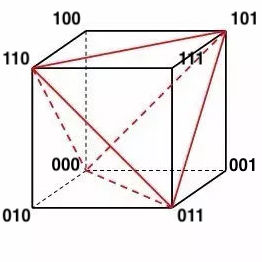
\includegraphics[width=6.00cm,height=6.00cm]{cube.jpg}
\caption{Tetrahedralization within a cube}
\end{figure}

\subsection{Compute Screen Space Projection Coordinate}
In this stage, we calculate every vertex’s screen space coordinate (SSC) in order to tell which tetrahedron(s) does a single pixel cover. Firstly we have known that Camera has a unit vector m\_Forward(CO) pointing at the center of film, two vectors m\_Right and m\_Up as the graph shows with magnitude of half of physical length and width of the film. Given a vertex v in the view, we have its screen projection P with 

\begin{equation} 
\boldsymbol {CP} = t 
\cdot
\boldsymbol{CV}
\quad (0<t<1)
\end{equation} 

Derive t by solving 

\begin{equation} 
\boldsymbol {CO}
\cdot 
\boldsymbol{OP}=0
\end{equation} 

since m\_Forward is always orthogonal to the screen by initial construction. Then we calculate OP’s projection on m\_Right and m\_Up to obtain its coordinate, and subsequently the coordinate with respect to pixel (e.g lower left corner’s pixel point(0,0), up right corner’s pixel point(1023,1023)). 
\\
\subsection{Extract Intersection Records}
The screen space projection of tetrahedra is implemented in this step. Since screen space projection of vertices have already been calculated and stored in SSC, we can directly access the projected 2D coordinates of the 4 vertices of a tetrahedron via vertex index. By inspection, the projected shape of a tetrahedron can be either a quardrilateral or a triangle(a concave quardrilateral).
\\The purpose of screen space projection of tetrahedra is to find out all tetrahedra a ray shooting from a specific pixel intersected with. Every pixel covered by the projected shape of a tetrahedron is considered affected by this tetrahedron in pixel color.
\\Before we project tetrahedra, a few helper functions are need to simplify our processing.
\\
\subsubsection{Helper function: cross product}
Cross product function basically takes in 2 2D vectors 
\textbf {vA},\textbf {vB}, then return a scalar

\begin{equation} 
\boldsymbol {vA}.x \cdot 
\boldsymbol {vB}.y - 
\boldsymbol {vB}.x \cdot 
\boldsymbol {vA}.y
\end{equation} 

This function is important and have been used a lot in following parts. 
\\
\subsubsection{Helper function: the side of line}
Given a line shooting from point \emph{pA} to point \emph{pB}, we need to decide whether point \emph{pC} is above the line or below the line. This is achieved by cross product $\overrightarrow{CA}$ and $\overrightarrow{AB}$. If the result > 0, then \emph{pC} is above the line; if the result = 0, \emph{pC} is on the line; if the result < 0, \emph{pC} is below the line.
\\
\subsubsection{Helper function: point inside triangle}
We need to decide whether a point \emph{pP} is inside a triangle connnected by \emph{pA}, \emph{pB} and \emph{pC}. This is easily achieved by justifing \emph{pP} and \emph{pA} are on the same side of $\overrightarrow{pBpC}$, \emph{pP} and \emph{pB} are on the same side of $\overrightarrow{pApC}$, \emph{pP} and \emph{pC} are on the same side of $\overrightarrow{pApB}$.
\\
\subsubsection{Case1: the projection is a triangle}
By testing whether there exists one of the four projected vertices of a tetrahedra inside the triangle formed by the rest of 3 vertices, we can easily find out whether the projection is a triangle or a quardrilateral.
\\If the projection is a triangle, we can easily decide what pixels are inside this triangle and then push this tetrahedron to the \textbf{PerPixelIntersectionList}.
\\To narrow the range of pixels to be decided, we only test pixels inside a square ranging from the minimum of x,y coordinates of the four vertices to the maximum of x,y coordinates.
\\
\subsubsection{Case2: the projection is a quardrilateral}
If the projection is a quardrilateral, the deciding process is a little bit complex. First of all, we need to find the correct connecting order of the 4 vertices clockwise. This can be achieved by finding out the leftmost and rightmost points \emph{pL}, \emph{pR}, then do $\overrightarrow{pLpR}$ line\_side test for the rest 2 vertices.
\\Now that we have \emph{pA},\emph{pB},\emph{pC},\emph{pD} 4 vertices clockwise, a popular method to decide whether pixel \emph{pP} is inside the quardrilateral is to do cross product $\overrightarrow{pApB}$ and $\overrightarrow{pApP}$, $\overrightarrow{pBpC}$ and $\overrightarrow{pBpP}$, $\overrightarrow{pCpD}$ and $\overrightarrow{pCpP}$, $\overrightarrow{pDpA}$ and $\overrightarrow{pDpP}$ separately, and test whether the second vector is on the clock wise direction of the first vector. If all of the above conditions are true, then \emph{pP} is inside quardrilateral \textbf{pApBpCpD}. Push this tetrahedron to \textbf{PerPixelIntersectionList}.
\\
\subsection{Sort Intersection Effect List in Ascending Order by Distance}
We have calculated the intersection effect of a tetrahedron for the specific pixel. Since the composition step composites all tetrahedron effects from the nearest to the farthest (similar to rendering from front to back in our assignment), we sort the \textbf{IntersectionEffect} list in ascending order by its distance. This is achieved by the sort function from the standard library.
\\
\subsection{Tetrahedralization}
To composite, for each pixel, we iterate its already sorted intersection effect list.
For each intersection, we update the destination color and opacity as the following equations:

\begin{gather} 
C_{color} = C_{color} + (1 - C_{opacity}) \cdot R_{color}\\
C_{opacity} = C_{opacity} + (1 - C_{opacity}) \cdot R_{opacity}
\end{gather}

Note that when the opacity is too high, we break the loop and stop composition.




\section{Results}






\end{document}
